\newpage
\section{SPICE}

\label{SPICE}
\begin{figure}[h]
\centering
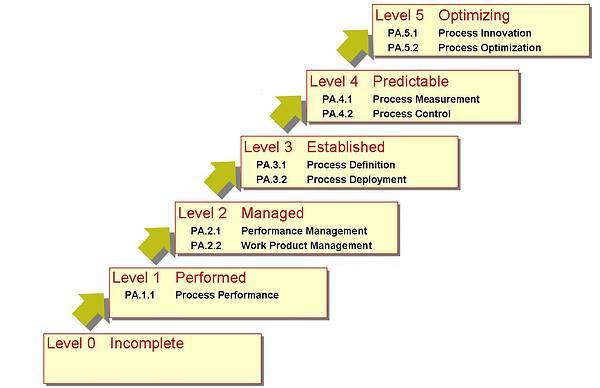
\includegraphics[scale=1,keepaspectratio]{SPICE.jpg}
\caption{SPICE}
\end{figure}
\FloatBarrier

Lo standard \textit{ISO/IEC 15504}\ped{G}, anche noto come SPICE (Software Process Improvement and Capability dEtermination), definisce un modello di riferimento per la valutazione del livello di maturità dei processi. \\ 
Per l'esattezza sono previsti sei livelli di maturità, per i quali vengono definiti degli attributi che permettano di misurarla:
\begin{itemize}
\item\textbf{Level 0 - Incomplete process}: il processo non è implementato o non riesce a raggiungere i suoi obiettivi;
\item\textbf{Level 1 - Performed process}: il processo viene messo in atto e raggiunge i suoi scopi. Viene misurato tramite:
\begin{itemize}
\item\textbf{Process performance}: capacità di raggiungere i propri obiettivi e di ottenere risultati identificabili.
\end{itemize}
\item\textbf{Level 2 - Managed process}: il processo viene eseguito sulla base di obiettivi ben definiti. Viene misurato tramite:
\begin{itemize}
\item\textbf{Performance management}: capacità di elaborare un prodotto coerente con gli obiettivi attesi;
\item\textbf{Work product management}: capacità di elaborare un prodotto appropriatamente documentato, controllato e verificato.
\end{itemize}
\item\textbf{Level 3 - Established process}: il processo viene eseguito in base ai principi dell’ingegneria del software. Viene misurato tramite:
\begin{itemize}
\item\textbf{Process definition}: capacità di raggiungere i propri obiettivi aderendo agli standard;
\item\textbf{Process resource}: capacità di sfruttare risorse adeguate che gli permettano di essere attuato efficacemente.
\end{itemize}
\item\textbf{Level 4 - Predictable process}: Il processo è attuato all'interno di limiti ben definiti. Viene misurato tramite:
\begin{itemize}
\item\textbf{Process measurement}: capacità di utilizzare i risultati raggiunti e le misure ricavate durante l'esecuzione per per garantire il raggiungimento dei traguardi definiti;
\item\textbf{Process control}: capacità di correggere o migliorare, se necessario,  le sue modalità di esecuzione, in seguito a controlli basati sulle misurazioni rilevate.
\end{itemize}
\item\textbf{Level 5 - Optimizing process}: Il processo è predicibile ed in grado di adattarsi per raggiungere obiettivi specifici e rilevanti. Viene misurato tramite:
\begin{itemize}
\item\textbf{Process change}: capacità di tenere sotto controllo tutti i cambiamenti strutturali e di esecuzione;
\item\textbf{Continuous improvement}: capacità di identificare
e implementare le modifiche effettuate, per garantire un miglioramento continuo nella realizzazione degli obiettivi fissati.
\end{itemize}
\end{itemize} 	

Ogni attributo definito precedentemente è misurabile e lo standard stabilisce
4 differenti livelli:
\begin{itemize}
\item\textbf{N}: non posseduto (0\% - 15\%);
\item\textbf{P}: parzialmente posseduto (16\% - 50\%);
\item\textbf{L}: largamente posseduto (51\% - 85\%);
\item\textbf{F}: completamente posseduto (86\% - 100\%).
\end{itemize}